\documentclass[{../../master}]{subfiles}
\graphicspath{{../..}}  % 個別コンパイル時の画像パスを解決する

\begin{document}

\section{被覆付圧着端子の付け方}

ADAMR2では,スイッチや端子台との接続に被覆付圧着端子を使用しています.
被覆付圧着端子を配線ケーブルに取り付ける際は,裸圧着端子よりも多くのことに気を付けなければなりません.
ここでは被覆付圧着端子を取り付ける際の手順と注意点を説明します.

\subsection{使用する端子とケーブルについて}

ADAMR2で使用する配線部品を表\ref{tab:list_of_wiring_components}に示します.

\begin{table}[ht]
  \begin{center}
    \begin{tabular}{|l|l|}
      \hline
      Name & Model Number \\ \hline
      ニチフ 銅線用絶縁被覆付圧着端子丸型 & TMEV1.25-3 \\ \hline
      差込み型接続端子 187シリーズ(バリュー品) メス(嵌合部絶縁型) & MTR-480809-FA \\ \hline
      絶縁付圧着端子 Y型 & F1.25-5 \\ \hline
      通信機器用ビニル電線 KVシリーズ & KV 1.25SQ アカ-200 \\ \hline
      通信機器用ビニル電線 KVシリーズ & KV 1.25SQ クロ-200 \\ \hline
    \end{tabular}
  \end{center}
  \caption{List of Wiring Components}
  \label{tab:list_of_wiring_components}
\end{table}

使用する配線ケーブルは太さAWG16(sq1.25)の撚線ビニル電線です.
被覆付圧着端子は,内径$\phi$\SI{3}{mm}の丸型圧着端子,187サイズの差込型接続端子,内径$\phi$\SI{5}{mm}のY型圧着端子の3種類です.
いずれもAWG16サイズの電線に対応しているものを使用します.

\subsection{必要な工具}

配線には以下の工具が必要となります.

\begin{itemize}
  \item 圧着工具
  \item ワイヤーストリッパー
  \item ニッパー
  \item 電工ペンチ
\end{itemize}

被覆付圧着端子をケーブルに取り付けるには,専用の工具が必要となります.
ここではホーザン株式会社のの絶縁被覆付圧着端子用圧着工具P-743を使用しました.

\begin{figure}[ht]
  \centering
  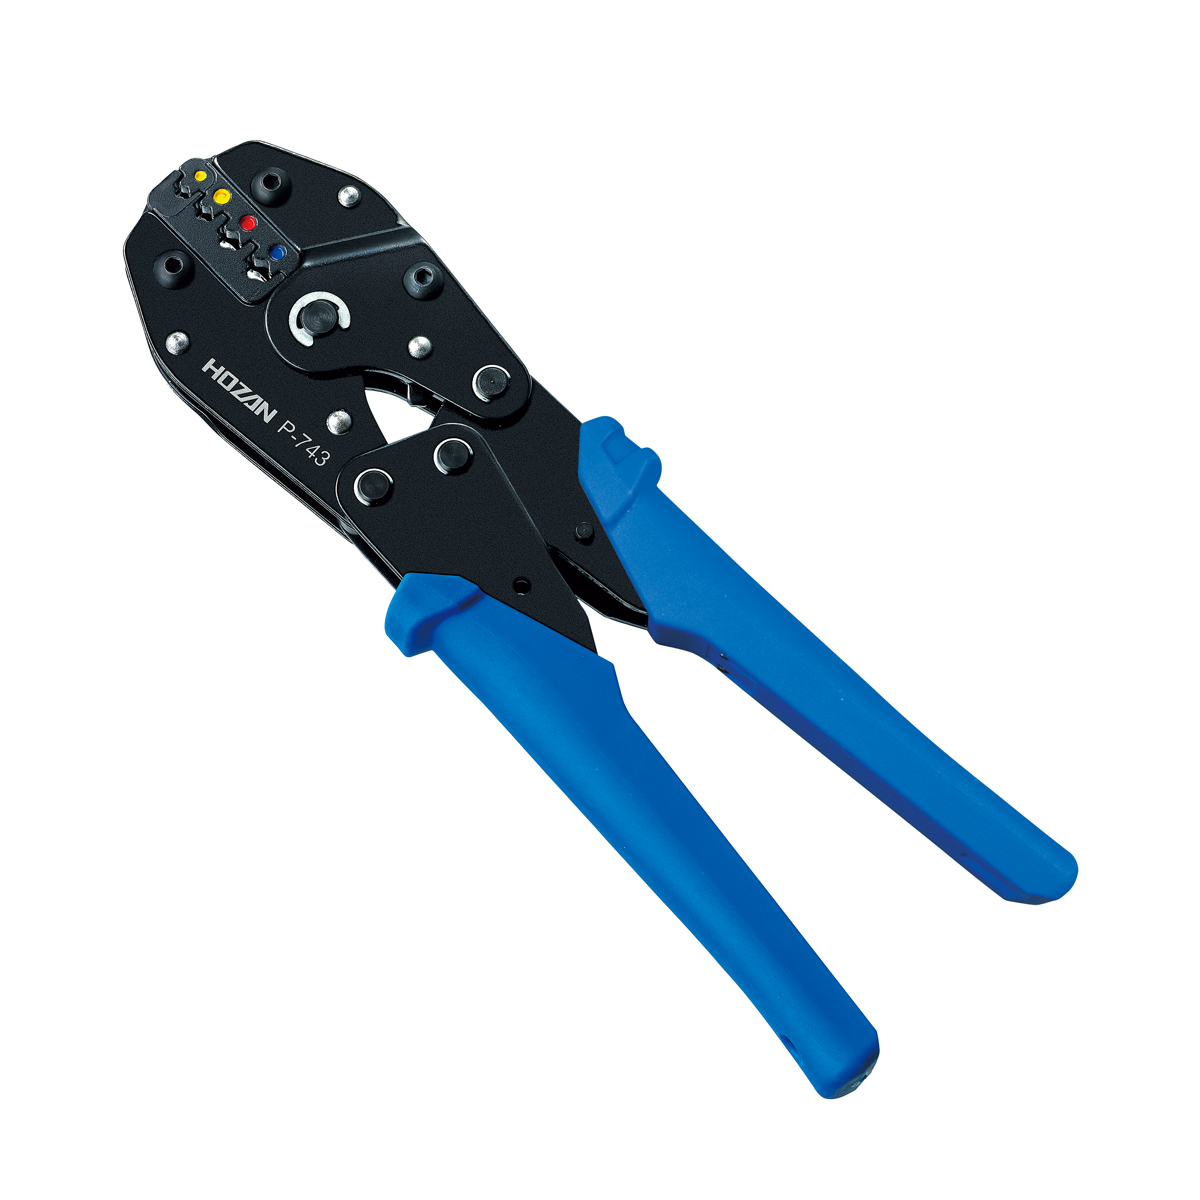
\includegraphics[height=50truemm]{images/P-743.jpg}
  \caption{HOZAN P-743}
\end{figure}

ワイヤーストリッパーはホーザン株式会社のP-90-Aを使用しました.

\begin{figure}[ht]
  \centering
  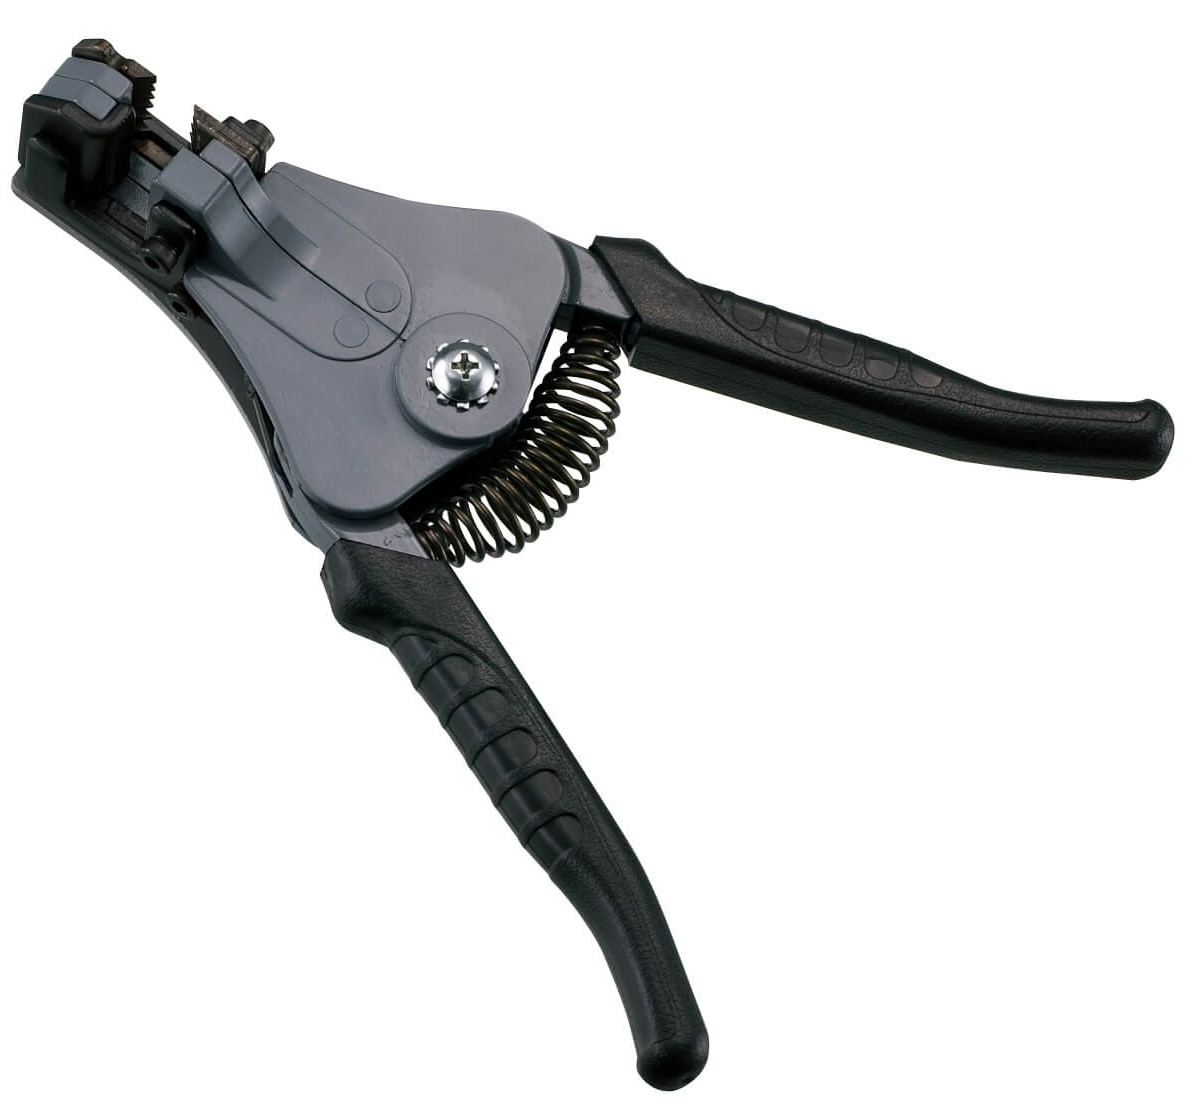
\includegraphics[height=50truemm]{images/P-90-series.jpg}
  \caption{HOZAN P-90-A}
\end{figure}

また,先端に被覆付圧着端子のためのカシメ部がついた電工ペンチがあると圧着を確実に行うことができるので,あった方が望ましいです.

\begin{figure}[ht]
  \centering
  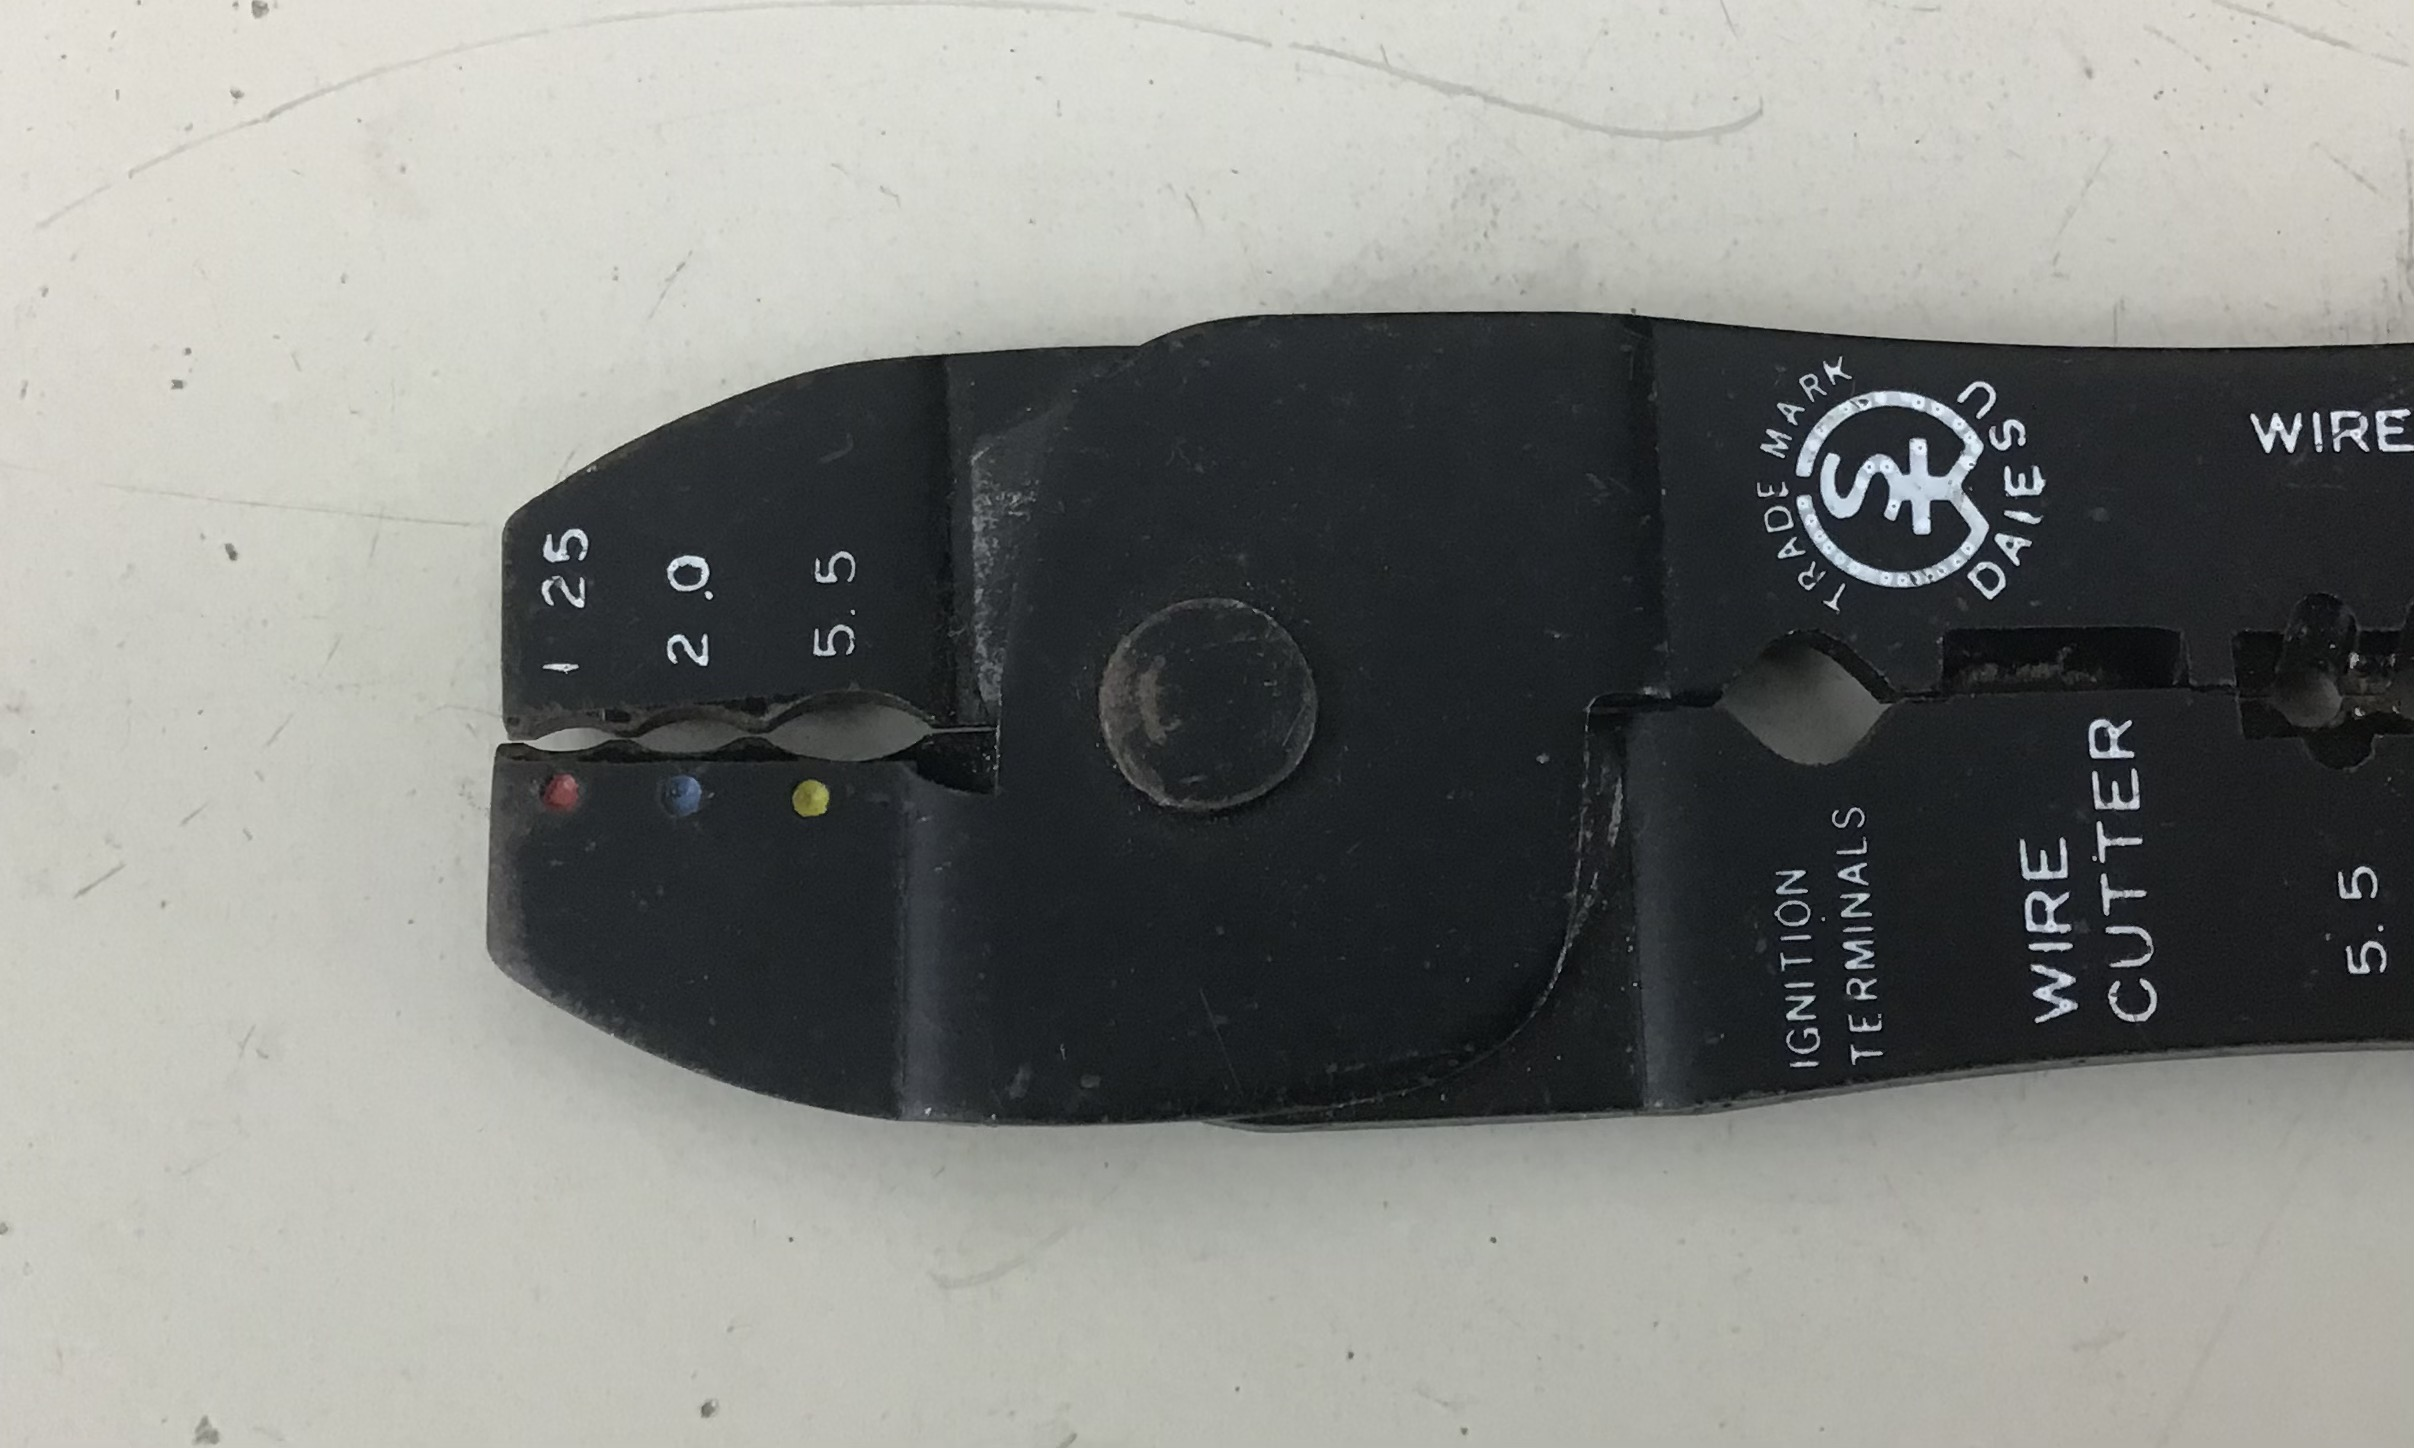
\includegraphics[height=50truemm]{images/crimp_plier.jpg}
  \caption{A Crimp Plier}
\end{figure}


\subsection{圧着の手順}

圧着端子の種類が違っても,作業手順はおおよそ同じです.
まずはケーブルの被覆を剥ぎます.
P-90-Aの\SI{1.6}{mm}のスロットを使うと綺麗に電線を剥ぐことができます.
およそ\SI{6}{mm}だけ被覆を剥ぐと,圧着をスムーズに行うことができます.

そして,ここが重要なのですが,圧着端子を付ける前に図\ref{fig:twist_the_wire}のように電線をねじって撚っておきます.
電線をねじっておくことで,圧着した際に端子との摩擦が増し,端子が外れにくくなります.
\footnote{電線をねじらずに圧着すると,特に差込型接続端子は簡単にすっぽ抜けます.}

\begin{figure}[ht]
  \centering
  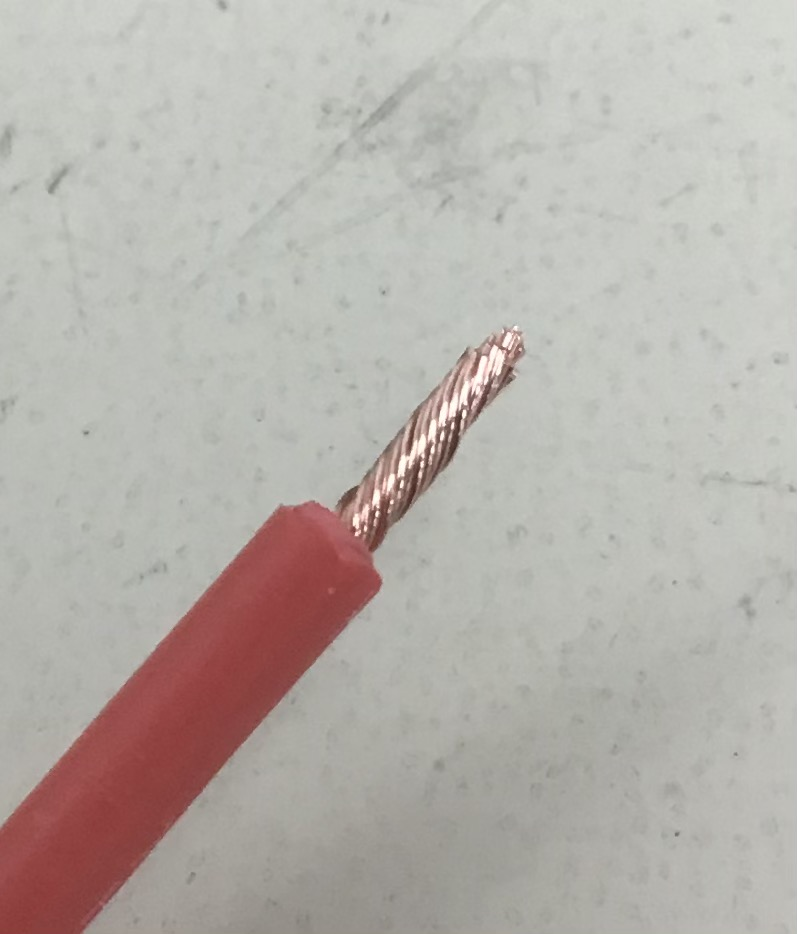
\includegraphics[height=50truemm]{images/twist_the_wire.jpg}
  \label{fig:twist_the_wire}
  \caption{Twist the Wire}
\end{figure}

電線の準備ができたら,圧着端子を挿入し,圧着工具のダイスにセットします.
今回使用する圧着端子のサイズはすべて1.25なので,P-743の赤色のマークが付いたダイスにセットします.
この時,圧着工具に端子をセットする際の向きに注意してください.正しい向きにセットしないと圧着が上手くいきません.
図\ref{fig:direction_for_setting_the_crimped_terminal}を参考に,正しい向きで端子をセットしてください.

\begin{figure}[ht]
  \centering
  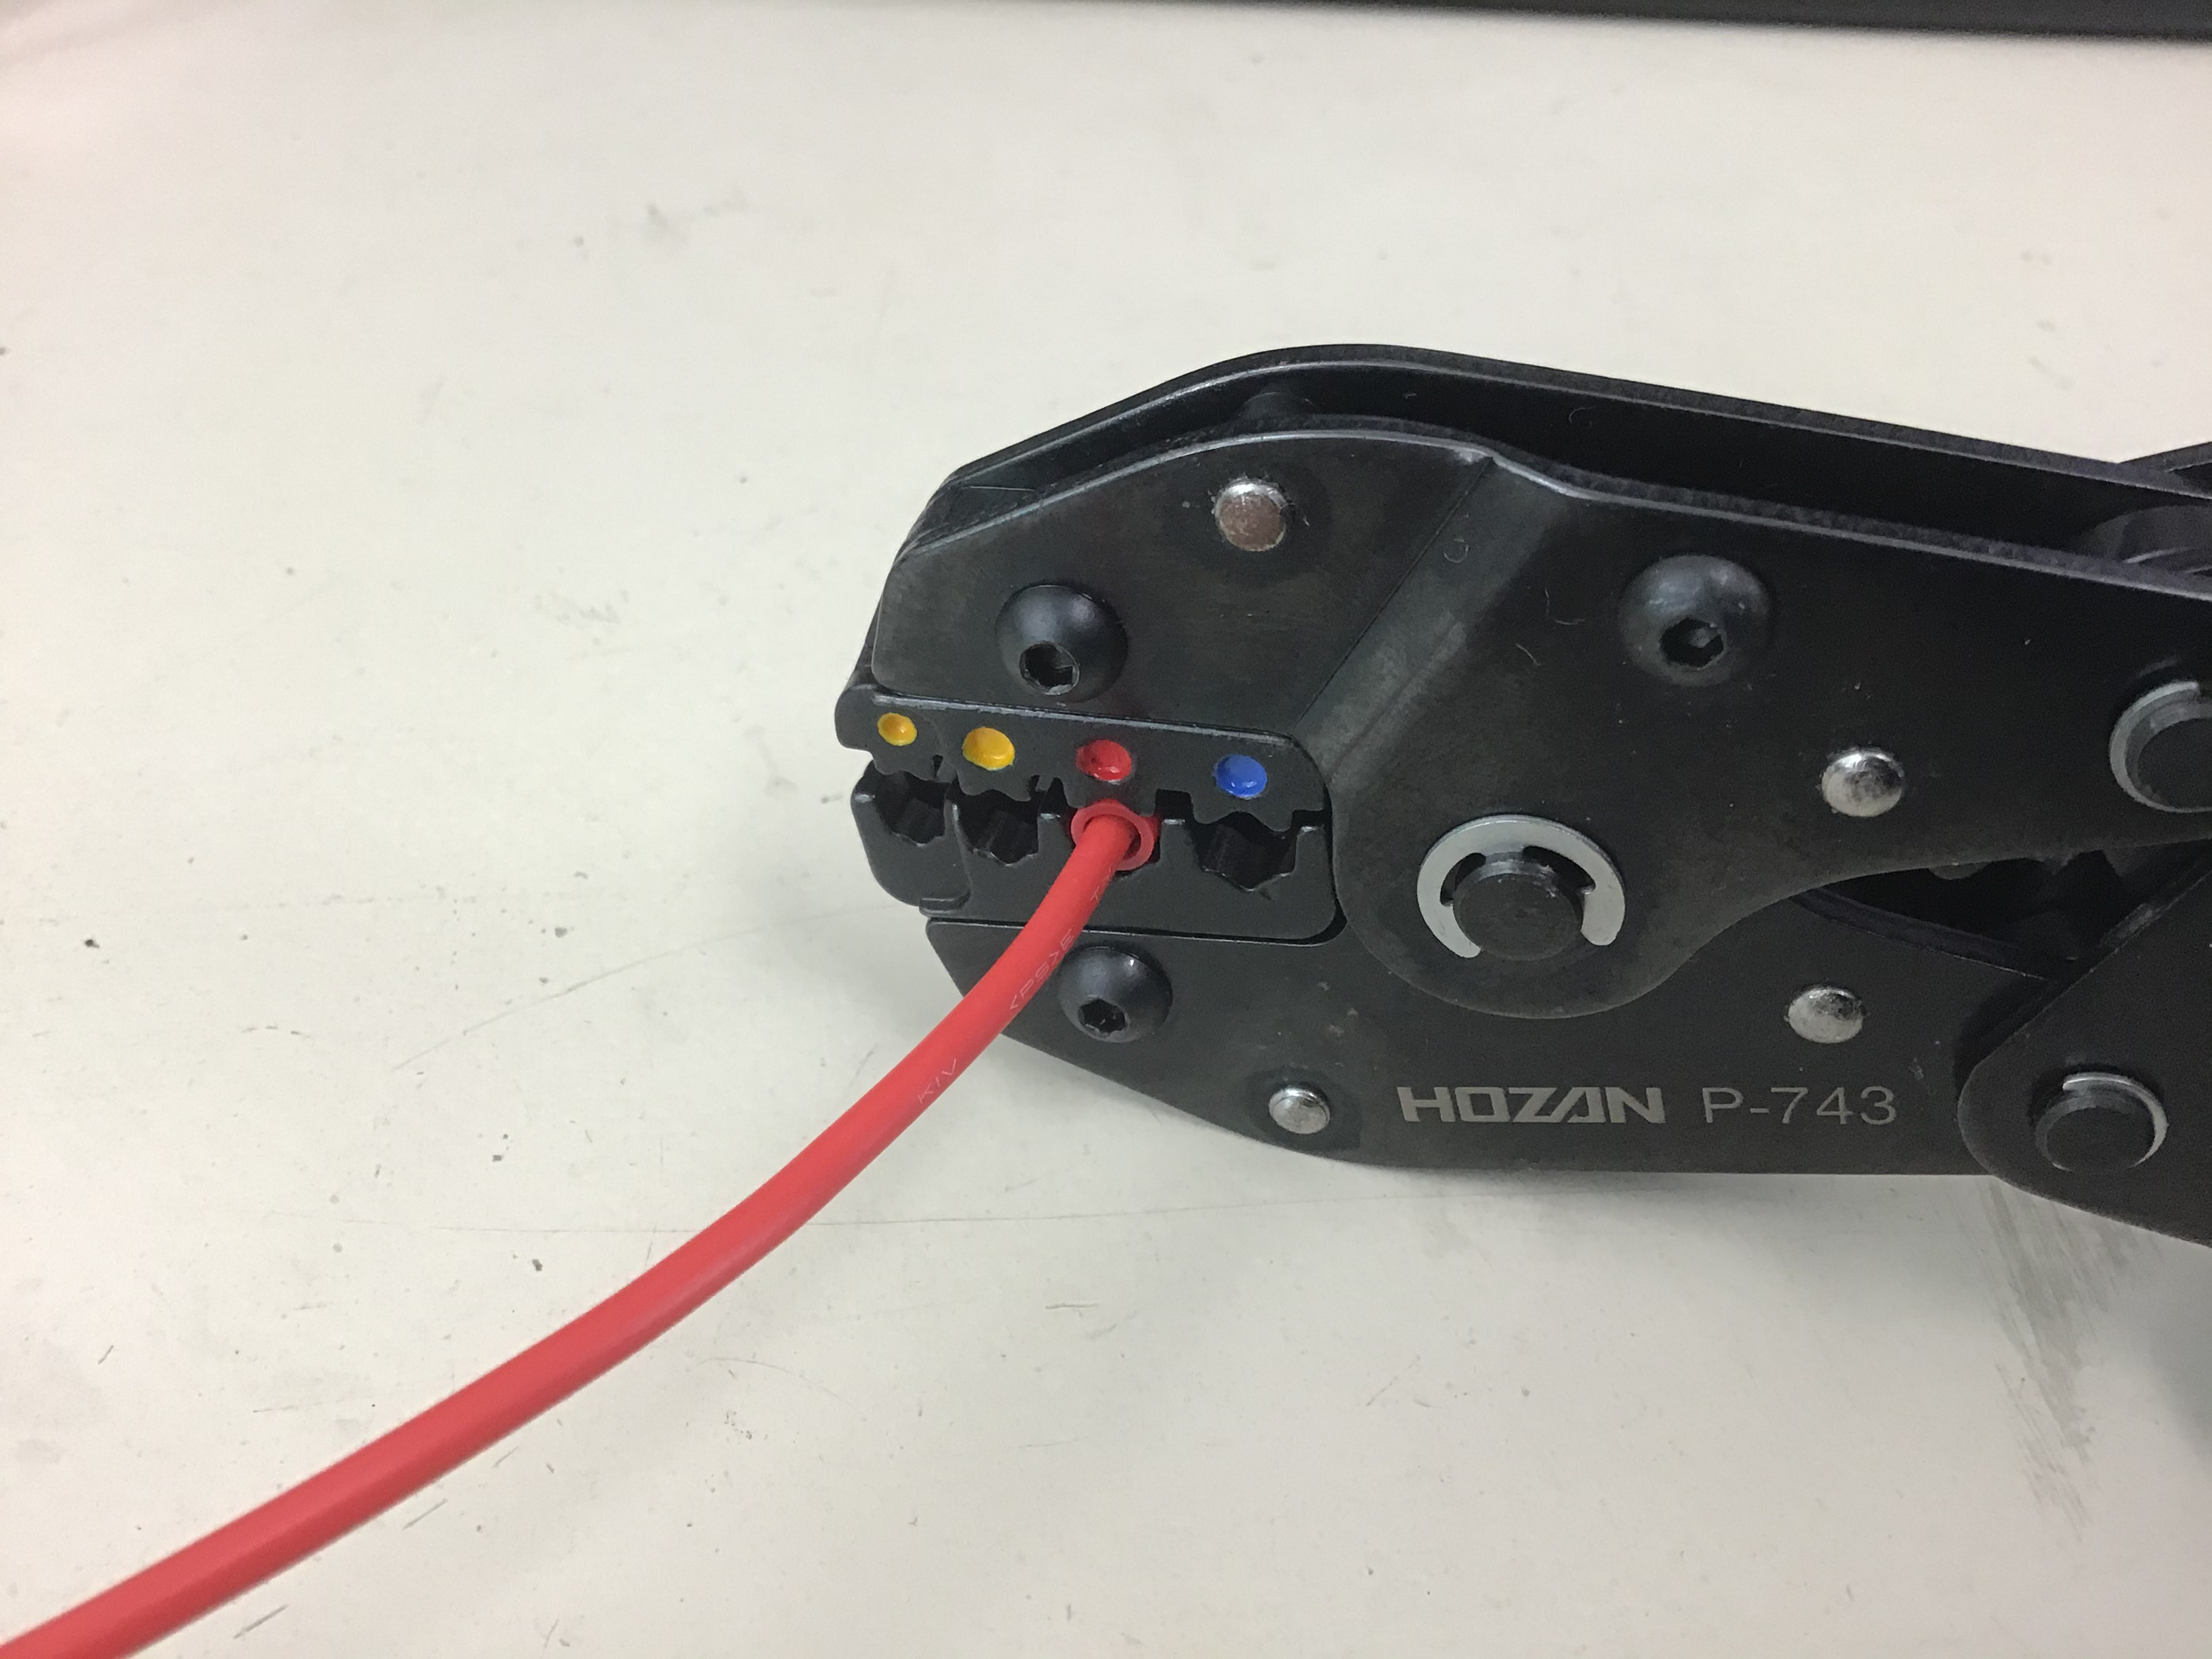
\includegraphics[height=50truemm]{images/direction_for_setting_the_crimped_terminal.jpg}
  \label{fig:direction_for_setting_the_crimped_terminal}
  \caption{Direction for Setting the Crimped Terminal}
\end{figure}

端子をダイスにセットしたら,ずれないように気を付けながらハンドルを握って圧着します.

丸型端子及びY型端子は,P-743による圧着だけでしっかりと圧着することができます.
しかし,差込型接続端子の場合はこれだけでは端子がすぐ抜けてしまう可能性があります.
\footnote{筆者が購入した差込型接続端子の品質に問題があったからかもしれません.}
そこで,P-743による圧着の後,電工ペンチを使ってさらに圧力をかけ,圧着を強くする必要があります.
かなり強めに力を込めて追い圧着すれば,すっぽ抜けてしまうことはなくなるはずです.

\begin{figure}[ht]
  \centering
  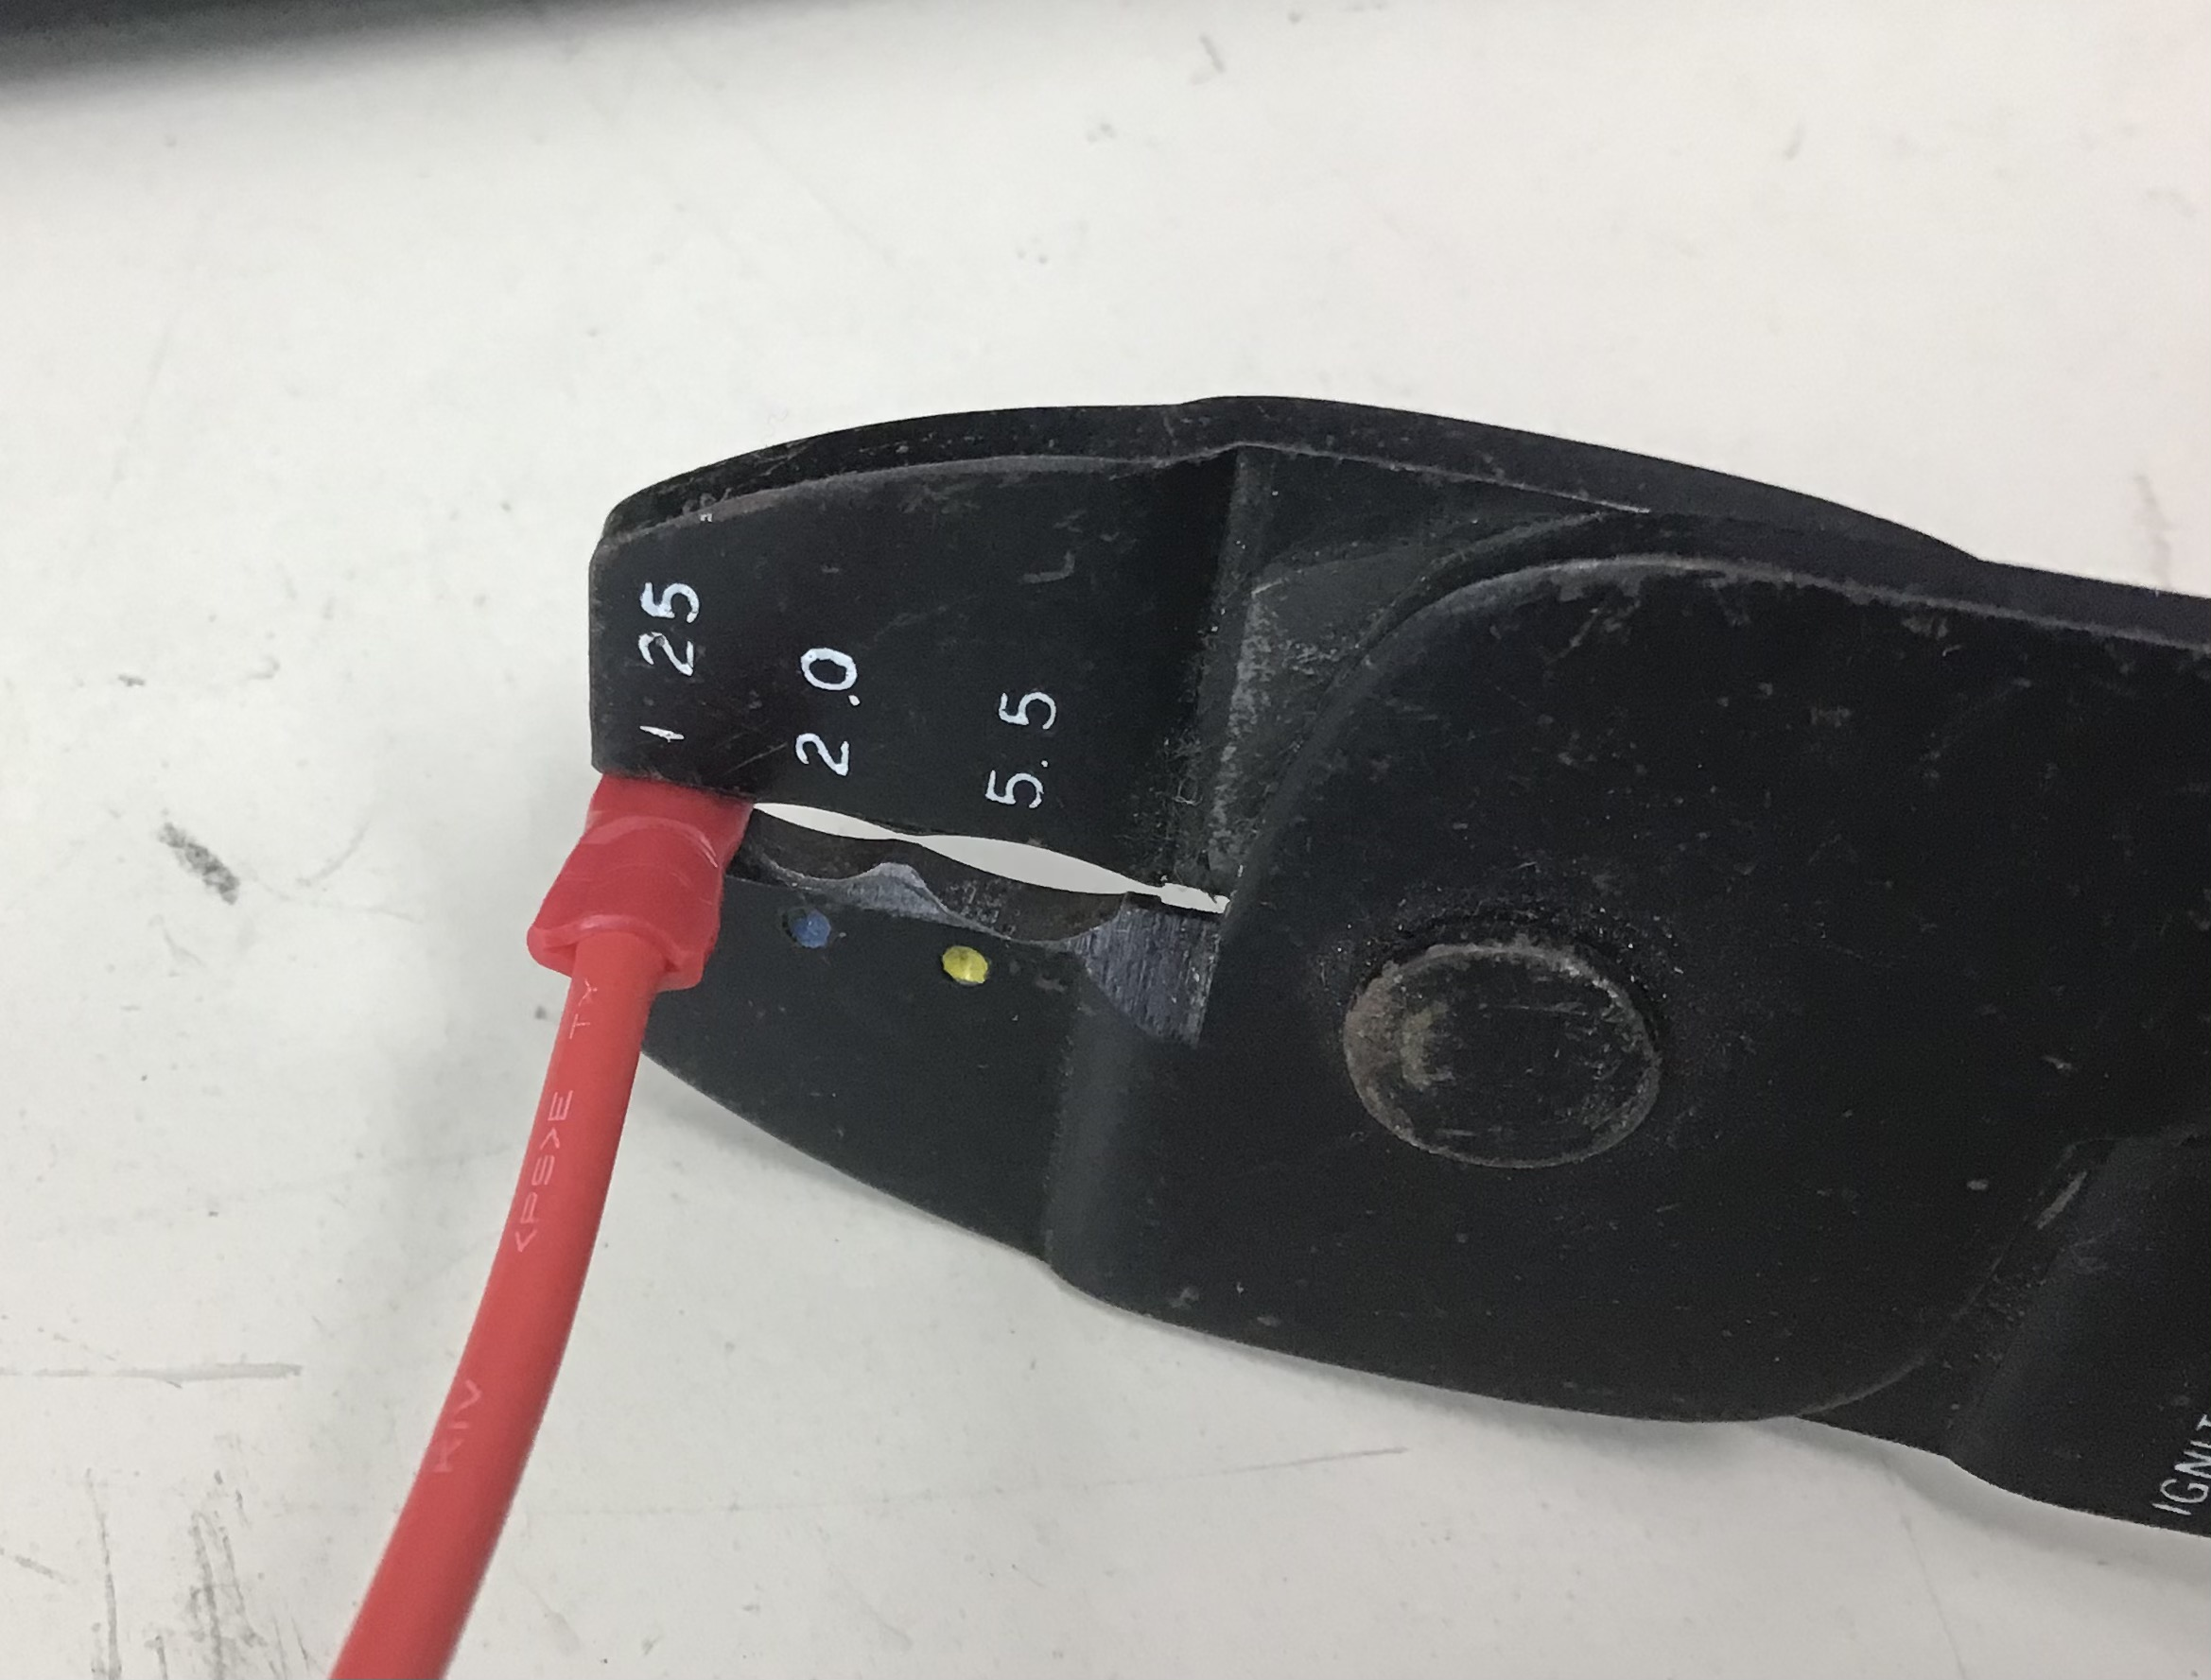
\includegraphics[height=50truemm]{images/crimp_further_with_crimp_plier.jpg}
  \label{fig:crimp_further_with_crimp_plier}
  \caption{Crimp Further with Crimp Plier}
\end{figure}

以上で圧着端子のケーブルへの取り付け作業は完了です.
圧着端子の取り付け方法に関しては,本ドキュメントだけでなく工具メーカーのページ等を参考に,正しい方法で作業を行うことを心掛けてください.

\end{document}